\chapter{Control of Gene Expression}\label{ch:b1:expression-control}

A bacterium growing on glucose carries five molecules of the \omterm{def:b1:enzymes:enzyme}{enzyme}
that digests lactose; give it lactose and, within minutes, it carries
five thousand. A liver \omterm{def:b1:cell-unit-of-life:cell}{cell} and a \omterm{def:b1:body-plans-tissues:nervous}{neuron} carry the same twenty
thousand \omterm{def:b1:genomes:gene}{genes} and make almost entirely different sets of \omterm{def:b1:proteins:peptide}{proteins},
and neither will ever make the other's. Nothing in
\cref{ch:b1:gene-expression} explains this: the machinery of
expression is the same for every \omterm{def:b1:genomes:gene}{gene}. What differs is whether a \omterm{def:b1:genomes:gene}{gene}
is read, how often, and for how long --- decisions taken at the
promoter by \omterm{def:b1:proteins:peptide}{proteins} that bind \omterm{def:b1:nucleic-acids:chain}{DNA}, and after it by the fate of the
messenger and the \omterm{def:b1:proteins:peptide}{protein}. This chapter describes how bacteria switch
\omterm{def:b1:genomes:gene}{genes} on and off in response to their food, how eukaryotes control
their \omterm{def:b1:genomes:gene}{genes} through chromatin, distant \omterm{def:b1:expression-control:enhancer}{enhancers} and combinations of
factors, and how the same control, applied to different \omterm{def:b1:genomes:gene}{genes} in
different \omterm{def:b1:cell-unit-of-life:cell}{cells}, makes a body out of one \omterm{def:b1:genomes:genome}{genome}.

\section{Why and where genes are controlled}

\begin{proposition}[Expression is regulated, at every level]\label{prop:b1:expression-control:levels}
\index{gene regulation}\index{constitutive gene}
Some \omterm{def:b1:genomes:gene}{genes} are \emph{constitutive} --- expressed always, at a steady
level, because their products are always needed (the \omterm{def:b1:gene-expression:ribosome}{ribosome}'s
\omterm{def:b1:proteins:peptide}{proteins}, the \omterm{def:b1:enzymes:enzyme}{enzymes} of \omterm{def:b1:respiration-fermentation:glycolysis}{glycolysis}). Most are \emph{regulated}:
expressed only in some conditions, some \omterm{def:b1:cell-unit-of-life:cell}{cells}, some moments. The
control acts at every step of the flow --- chiefly at the start of
transcription, the cheapest place to decide, but also at the
processing, export, stability and translation of the messenger, and
at the modification and degradation of the \omterm{def:b1:proteins:peptide}{protein} --- and the
response times range from seconds (a \omterm{def:b1:proteins:peptide}{protein} modified) through
minutes (a bacterial \omterm{def:b1:genomes:gene}{gene} switched on) to days (a chromatin state
changed).
\end{proposition}

\begin{example}[Making enzymes only when needed]\label{ex:b1:expression-control:economy}
The \omterm{def:b1:enzymes:enzyme}{enzyme} $\beta$-galactosidase, which splits lactose, is a tetramer
of four chains of \qty{1024}{} residues: five thousand copies are
\qty{3}{\%} of a \omterm{def:b1:cell-unit-of-life:cell}{cell}'s \omterm{def:b1:proteins:peptide}{protein} and cost \qty{8e7}{} \omterm{def:b1:water-small-molecules:atp}{ATP} per
generation. A bacterium that made them with no lactose to digest
would grow about one percent slower than a competitor that did not,
and in a few hundred generations would be outnumbered. Regulation is
selected because expression is expensive.
\end{example}

\section{The lac operon}

\begin{definition}[Operon, repressor, operator]\label{def:b1:expression-control:operon}
\index{operon}\index{repressor}\index{operator}\index{lac operon}
An \emph{operon} is a group of bacterial \omterm{def:b1:genomes:gene}{genes} transcribed together
from one promoter into one messenger, and so controlled together. The
\emph{lac operon} of \emph{E. coli} comprises three \omterm{def:b1:genomes:gene}{genes} for the use
of lactose --- \emph{lacZ} ($\beta$-galactosidase), \emph{lacY} (the
lactose permease that imports it) and \emph{lacA} --- behind a
promoter and an \emph{operator}, a short sequence overlapping the
promoter. A separate \omterm{def:b1:genomes:gene}{gene}, \emph{lacI}, makes the \emph{lac
repressor}, a \omterm{def:b1:proteins:peptide}{protein} that binds the operator and blocks the
polymerase. Lactose, converted in the \omterm{def:b1:cell-unit-of-life:cell}{cell} to allolactose, is the
\emph{inducer}: it binds the repressor, changes its shape, and makes
it let go of the operator. The operon is thus off unless lactose is
present --- \emph{negative control} lifted by \emph{induction}.
\end{definition}

\begin{omfigure}
\begin{tikzpicture}[font=\footnotesize, >=Stealth, line cap=round]
  % state 1: no lactose
  \begin{scope}
    \draw[very thick, gray] (0,0) -- (11,0);
    \fill[omExo!50] (0.2,-0.2) rectangle (1.6,0.2); \node[anchor=south, font=\scriptsize] at (0.9,0.25) {\emph{lacI}};
    \fill[omProp!50] (2.4,-0.2) rectangle (3.6,0.2); \node[anchor=north, font=\scriptsize] at (3.0,-0.25) {promoter};
    \fill[omThm!50] (3.6,-0.2) rectangle (4.4,0.2); \node[anchor=south, font=\scriptsize] at (4.0,0.25) {operator};
    \fill[omDef!60] (4.5,-0.2) rectangle (7.2,0.2); \node[anchor=south, font=\scriptsize] at (5.85,0.25) {\emph{lacZ}};
    \fill[omDef!60] (7.3,-0.2) rectangle (9.0,0.2); \node[anchor=south, font=\scriptsize] at (8.15,0.25) {\emph{lacY}};
    \fill[omDef!60] (9.1,-0.2) rectangle (10.3,0.2); \node[anchor=south, font=\scriptsize] at (9.7,0.25) {\emph{lacA}};
    \node[draw, thick, fill=omThm!25, rounded corners=3pt, inner sep=2pt] (rep) at (4.0,-0.95) {repressor};
    \draw[->, thick] (0.9,-0.25) -- (0.9,-0.95) -- (3.3,-0.95);
    \draw[thick] (rep) -- (4.0,-0.22);
    \node[draw, thick, fill=omProp!25, rounded corners=3pt, inner sep=2pt] at (2.2,0.9) {RNA polymerase};
    \node[font=\scriptsize, anchor=west] at (3.45,0.9) {blocked};
    \node[anchor=east, align=right] at (-0.2,0) {no lactose:\\ operon OFF};
  \end{scope}
  % state 2: lactose present
  \begin{scope}[yshift=-3.0cm]
    \draw[very thick, gray] (0,0) -- (11,0);
    \fill[omExo!50] (0.2,-0.2) rectangle (1.6,0.2);
    \fill[omProp!50] (2.4,-0.2) rectangle (3.6,0.2);
    \fill[omThm!50] (3.6,-0.2) rectangle (4.4,0.2);
    \fill[omDef!60] (4.5,-0.2) rectangle (7.2,0.2); \fill[omDef!60] (7.3,-0.2) rectangle (9.0,0.2); \fill[omDef!60] (9.1,-0.2) rectangle (10.3,0.2);
    \node[draw, thick, fill=omThm!25, rounded corners=3pt, inner sep=2pt] (rep2) at (4.0,-1.0) {repressor + inducer};
    \node[font=\scriptsize, anchor=west] at (5.6,-1.0) {released from the operator};
    \node[draw, thick, fill=omProp!25, rounded corners=3pt, inner sep=2pt] at (3.0,0.85) {RNA polymerase};
    \draw[->, very thick, omProp!80!black] (4.0,0.85) -- (10.3,0.85) node[midway, above, font=\scriptsize] {one messenger for the three genes};
    \node[anchor=east, align=right] at (-0.2,0) {lactose present:\\ operon ON};
  \end{scope}
\end{tikzpicture}

{\small The \omterm{def:b1:expression-control:operon}{lac operon}. Without lactose the \omterm{def:b1:expression-control:operon}{repressor} sits on the
operator and the polymerase cannot start; with lactose the inducer
pulls the \omterm{def:b1:expression-control:operon}{repressor} off and the three \omterm{def:b1:genomes:gene}{genes} are transcribed into one
messenger.}
\end{omfigure}

\begin{proposition}[The operon model]\label{prop:b1:expression-control:jacobmonod}
The lac \omterm{def:b1:genomes:gene}{genes} are controlled by a diffusible \omterm{def:b1:expression-control:operon}{repressor} acting on a
site adjacent to the \omterm{def:b1:genomes:gene}{genes}: control is negative, the \omterm{def:b1:expression-control:operon}{repressor} acts in
\emph{trans} (from anywhere in the \omterm{def:b1:cell-unit-of-life:cell}{cell}), and the operator acts in
\emph{cis} (only on the \omterm{def:b1:genomes:gene}{genes} next to it).
\end{proposition}
\begin{proof}[Evidence]
Jacob and Monod (1959--1961) reasoned from mutants. Strains mutant in
\emph{lacI} ($I^-$) made the \omterm{def:b1:enzymes:enzyme}{enzyme} with or without lactose
(\emph{constitutive}); a normal \emph{lacI} \omterm{def:b1:genomes:gene}{gene} introduced on a second
copy of the region restored regulation, so the \omterm{def:b1:genomes:gene}{gene}'s product is a
diffusible \omterm{def:b1:expression-control:operon}{repressor} that a mutant lacks. Strains mutant in the
operator ($O^c$) were also constitutive, but a second normal operator
on another copy did not restore regulation --- the operator only
controls the \omterm{def:b1:genomes:gene}{genes} physically attached to it, so it is a site, not a
product. A third class ($I^s$) could not be induced at all, and was
dominant: a \omterm{def:b1:expression-control:operon}{repressor} that no longer binds the inducer. In the PaJaMo
experiment (1959) a normal \emph{lacI} \omterm{def:b1:genomes:gene}{gene} transferred by conjugation
into an $I^-$ \omterm{def:b1:cell-unit-of-life:cell}{cell} shut off the \omterm{def:b1:enzymes:enzyme}{enzyme} synthesis within minutes: the
\omterm{def:b1:expression-control:operon}{repressor} acts fast, and on transcription --- the messenger was later
shown to have a half-life of minutes.
\end{proof}

\begin{definition}[Positive control: CAP and cAMP]\label{def:b1:expression-control:cap}
\index{catabolite repression}\index{diauxie}
The lac promoter is weak: even without the \omterm{def:b1:expression-control:operon}{repressor}, the polymerase
starts rarely unless a second \omterm{def:b1:proteins:peptide}{protein}, \emph{CAP} (catabolite activator
\omterm{def:b1:proteins:peptide}{protein}), is bound just upstream of it, bending the \omterm{def:b1:nucleic-acids:chain}{DNA} and holding
the polymerase in place. CAP binds \omterm{def:b1:nucleic-acids:chain}{DNA} only when carrying
\emph{cyclic AMP}, whose level in the \omterm{def:b1:cell-unit-of-life:cell}{cell} falls when glucose is
abundant. The \omterm{def:b1:expression-control:operon}{operon} is therefore fully on only when lactose is
present \emph{and} glucose is absent: two signals, one negative and
one positive, are integrated at one promoter. Given both sugars,
\emph{E. coli} eats the glucose first, pauses while cAMP rises and
the lac \omterm{def:b1:enzymes:enzyme}{enzymes} are made, then eats the lactose --- the two-phase
growth curve called \emph{diauxie}, which Monod described in 1941 and
which set him on the road to the \omterm{def:b1:expression-control:operon}{operon}.
\end{definition}

\begin{omfigure}
\begin{tikzpicture}
\begin{semilogyaxis}[
  width=0.86\linewidth, height=6.0cm,
  axis x line=bottom, axis y line=left,
  xmin=0, xmax=6, ymin=1e7, ymax=3e9,
  xlabel={time (h)}, ylabel={cells per mL},
  xlabel style={font=\small, at={(axis description cs:0.5,-0.12)}, anchor=north},
  ylabel style={font=\small},
  tick label style={font=\small}, xtick={0,1,2,3,4,5,6},
  clip=false,
]
\addplot[very thick, omDef, domain=0:2, samples=30] {1e7*2^(x/0.333)};
\addplot[very thick, omDef, domain=2:2.6, samples=5] {6.4e8};
\addplot[very thick, omDef, domain=2.6:4.0, samples=30] {6.4e8*2^((x-2.6)/0.5)};
\addplot[very thick, omDef, domain=4.0:6, samples=5] {6.4e8*2^(1.4/0.5)};
\node[font=\scriptsize, anchor=north west, align=left] at (axis cs:0.15,8e8) {phase 1: glucose\\ (doubling \qty{20}{min})};
\node[font=\scriptsize, anchor=south, align=center] at (axis cs:2.3,7e8) {lag: cAMP rises,\\ lac enzymes made};
\node[font=\scriptsize, anchor=north west, align=left] at (axis cs:3.0,9e8) {phase 2: lactose\\ (doubling \qty{30}{min})};
\node[font=\scriptsize, anchor=south west] at (axis cs:4.1,4.4e9) {};
\end{semilogyaxis}
\end{tikzpicture}

{\small Diauxic growth of \emph{E. coli} on glucose plus lactose.
The culture grows on glucose alone, stops when it runs out, and
resumes on lactose after the half-hour it takes to induce the \omterm{def:b1:expression-control:operon}{lac
operon}.}
\end{omfigure}

\begin{omfigure}
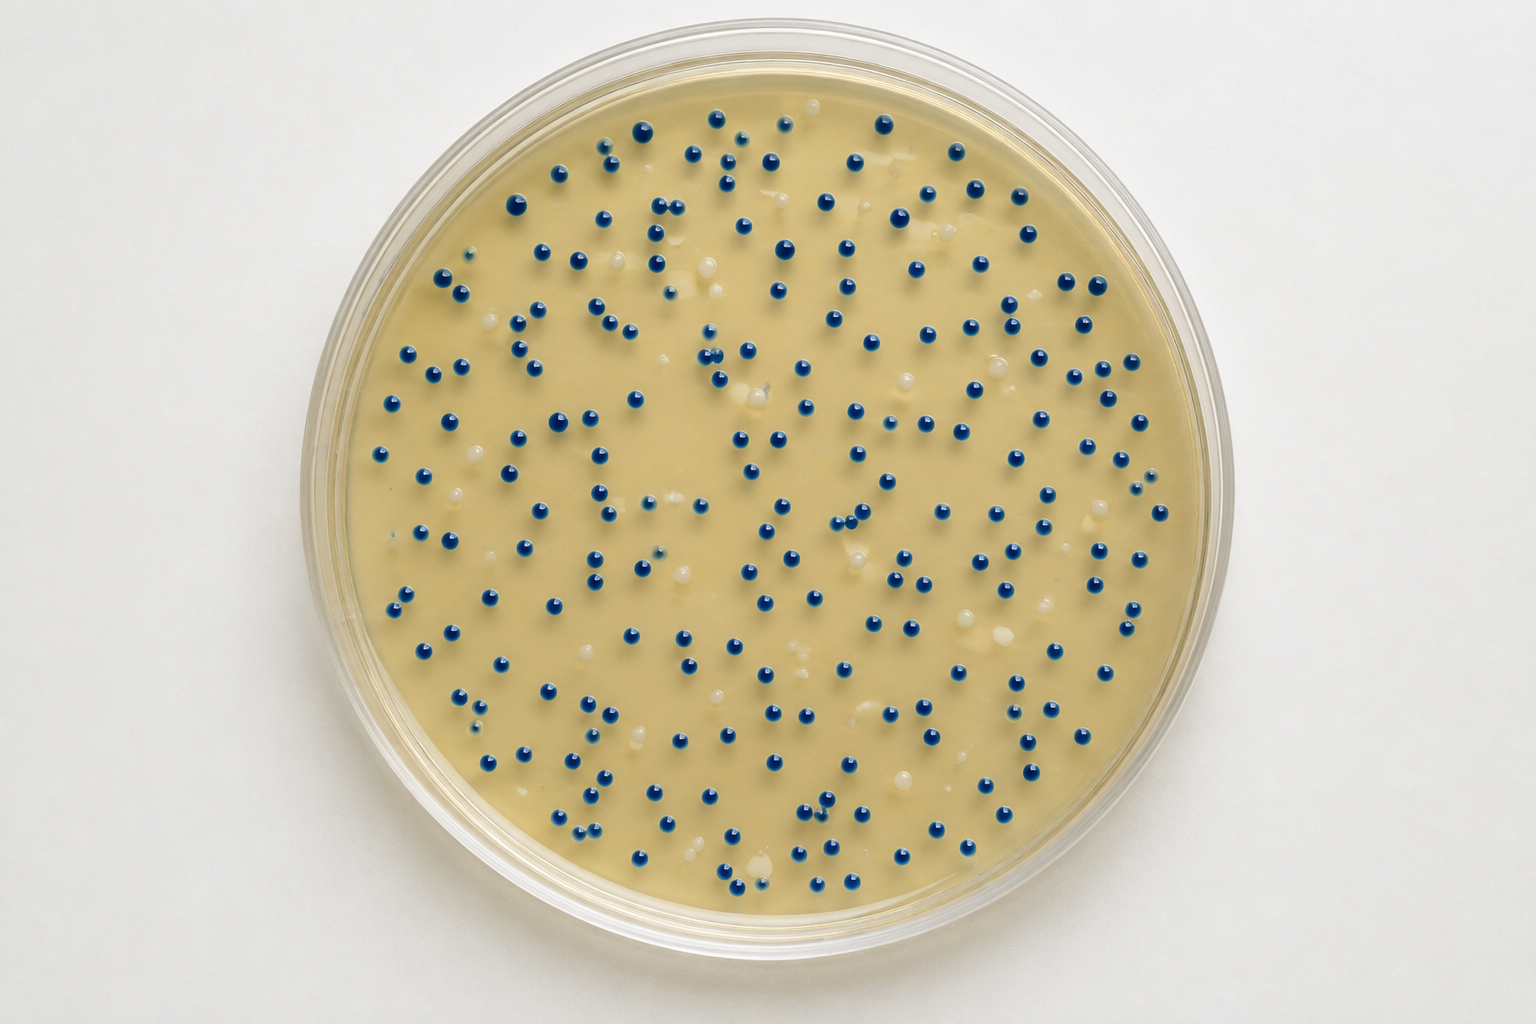
\includegraphics[width=0.46\linewidth]{images/book3/ai/b3-20-xgal-plate.png}

{\small The \omterm{def:b1:expression-control:operon}{lac operon} made visible: colonies on a plate containing
X-gal, a colourless substrate that $\beta$-galactosidase turns blue.
Blue colonies express \emph{lacZ}; white ones carry a broken \omterm{def:b1:genomes:gene}{gene} ---
the reporter used in a thousand experiments.}
\end{omfigure}

\begin{method}[Predicting a lac phenotype]\label{met:b1:expression-control:lacphenotype}
\begin{enumerate}
  \item Write the genotype of each copy of the region: $I$, $P$, $O$,
        $Z$ ($^+$ normal, $^-$ inactive, $O^c$ operator-constitutive,
        $I^s$ \omterm{def:b1:expression-control:operon}{super-repressor}).
  \item The \omterm{def:b1:expression-control:operon}{repressor} acts in trans: one $I^+$ anywhere represses
        every normal operator; $I^s$ represses whatever the inducer.
  \item The operator and promoter act in cis: an $O^c$ frees only the
        $Z$ on its own \omterm{def:b1:nucleic-acids:chain}{DNA}; a $P^-$ silences only its own \omterm{def:b1:genomes:gene}{genes}.
  \item Ask, with and without inducer, whether each $Z^+$ \omterm{def:b1:genomes:gene}{gene} is
        transcribed; the phenotype is inducible, constitutive or
        uninducible accordingly. Then add glucose: without cAMP--CAP,
        transcription is low whatever the \omterm{def:b1:expression-control:operon}{repressor} does.
\end{enumerate}
\end{method}

\begin{example}[Two partial diploids]\label{ex:b1:expression-control:diploids}
$I^-\,O^+\,Z^+ / I^+\,O^+\,Z^-$: the $I^+$ copy makes \omterm{def:b1:expression-control:operon}{repressor} that
binds the $O^+$ next to $Z^+$; inducible --- the mutation is
complemented. $I^+\,O^c\,Z^+ / I^+\,O^+\,Z^-$: the only working $Z$
sits behind an operator the \omterm{def:b1:expression-control:operon}{repressor} cannot bind; constitutive --- the
normal operator on the other copy cannot help, since it controls only
the broken $Z$.
\end{example}

\section{Other bacterial strategies}

\begin{proposition}[Repression, attenuation and sigma factors]\label{prop:b1:expression-control:trp}
\index{trp operon}\index{attenuation}\index{sigma factor}
\omterm{def:b1:expression-control:operon}{Operons} for biosynthesis are controlled in the opposite sense: the
\emph{\omterm{prop:b1:expression-control:trp}{trp operon}}, five \omterm{def:b1:genomes:gene}{genes} for making tryptophan, is transcribed
unless tryptophan is present --- the \omterm{def:b1:proteins:aminoacid}{amino acid} binds the trp
\omterm{def:b1:expression-control:operon}{repressor} and \emph{enables} it to bind the operator (a corepressor).
A second, finer control, \emph{attenuation}, uses the coupling of
transcription and translation in bacteria: the start of the messenger
encodes a short peptide with two tryptophans in a row; if
tryptophan-loaded tRNA is abundant, a \omterm{def:b1:gene-expression:ribosome}{ribosome} translates it quickly
and the \omterm{def:b1:nucleic-acids:chain}{RNA} behind folds into a terminator hairpin that stops the
polymerase before the \omterm{def:b1:genomes:gene}{genes}; if tryptophan is scarce, the \omterm{def:b1:gene-expression:ribosome}{ribosome}
stalls at the tryptophan \omterm{def:b1:gene-expression:code}{codons} and the \omterm{def:b1:nucleic-acids:chain}{RNA} folds differently,
letting transcription continue. Bacteria also switch whole sets of
\omterm{def:b1:genomes:gene}{genes} by changing the $\sigma$ subunit of their polymerase: a
heat-shock $\sigma$ directs it to the promoters of chaperone \omterm{def:b1:genomes:gene}{genes}; a
sporulation $\sigma$ to those of spore formation.
\end{proposition}

\section{Control in eukaryotes}

\begin{definition}[Transcription factors, enhancers]\label{def:b1:expression-control:enhancer}
\index{transcription factor}\index{enhancer}
In eukaryotes the polymerase never starts by itself: the general
factors at the promoter (\cref{ch:b1:gene-expression}) recruit it, and
the rate is set by \emph{transcription factors} bound to
\emph{regulatory sequences} --- some near the promoter, many in
\emph{enhancers} that can lie thousands of \omterm{thm:b1:nucleic-acids:helix}{base pairs} away, upstream,
downstream or in an \omterm{def:b1:genomes:gene}{intron}, in either orientation, and act by
\emph{looping} the \omterm{def:b1:nucleic-acids:chain}{DNA} so that the factors bound on them touch the
promoter's complex through mediator \omterm{def:b1:proteins:peptide}{proteins}. A transcription factor
is modular: a \emph{DNA-binding domain} that recognises a short
sequence (helix-turn-helix, zinc finger, leucine zipper families)
and an \emph{activation} or \emph{repression domain} that recruits or
blocks the machinery. A \omterm{def:b1:genomes:gene}{gene} is read when the right \emph{combination}
of factors is present: a few hundred factors, in combinations, control
twenty thousand \omterm{def:b1:genomes:gene}{genes}.
\end{definition}

\begin{omfigure}
\begin{tikzpicture}[font=\footnotesize, >=Stealth, line cap=round]
  % DNA with enhancer far upstream, looped to promoter
  \draw[very thick, gray] (0,0) -- (2.2,0) .. controls (3.2,0) and (3.4,2.6) .. (5.0,2.6) .. controls (6.6,2.6) and (6.8,0) .. (7.8,0) -- (12.5,0);
  \fill[omExo!60] (0.4,-0.2) rectangle (2.0,0.2); \node[anchor=north, font=\scriptsize] at (1.2,-0.25) {enhancer (\qtyrange{1}{100}{kb} away)};
  \fill[omProp!50] (8.0,-0.2) rectangle (9.4,0.2); \node[anchor=north, font=\scriptsize] at (8.7,-0.25) {promoter};
  \fill[omDef!60] (9.5,-0.2) rectangle (12.3,0.2); \node[anchor=north, font=\scriptsize] at (10.9,-0.25) {gene};
  % looped enhancer brought near promoter: draw factors at the loop apex near promoter? Simplify: activators on enhancer, mediator bridging
  \node[draw, thick, fill=omExo!30, rounded corners=3pt, inner sep=2pt] (act) at (1.2,0.75) {activators};
  \node[draw, thick, fill=omThm!25, rounded corners=3pt, inner sep=2pt, align=center] (med) at (5.0,1.5) {mediator};
  \node[draw, thick, fill=omProp!30, rounded corners=3pt, inner sep=2pt, align=center] (pol) at (8.7,0.85) {general factors\\ + polymerase};
  \draw[thick, omExo!80!black] (act) -- (2.4,1.2) -- (med);
  \draw[thick, omThm] (med) -- (pol);
  \node[anchor=north, align=center, gray] at (6.2,-1.0) {the DNA loops so that factors bound far away touch the promoter complex;\\ a gene is read when the right combination of factors is bound};
\end{tikzpicture}

{\small \omterm{def:b1:expression-control:enhancer}{Enhancer} action. Activators bound to a distant \omterm{def:b1:expression-control:enhancer}{enhancer} are
brought to the promoter by looping of the \omterm{def:b1:nucleic-acids:chain}{DNA}, and a mediator complex
relays their signal to the polymerase.}
\end{omfigure}

\begin{proposition}[Chromatin is part of the control]\label{prop:b1:expression-control:chromatin}
\index{histone acetylation}\index{DNA methylation}
A \omterm{def:b1:genomes:gene}{gene} wrapped in \omterm{def:b1:genomes:nucleosome}{nucleosomes} packed into heterochromatin cannot be
read: the factors cannot reach it. Activators recruit \omterm{def:b1:enzymes:enzyme}{enzymes} that
\emph{acetylate} the \omterm{def:b1:genomes:nucleosome}{histones}, loosening their grip on the \omterm{def:b1:nucleic-acids:chain}{DNA} and
marking the region as open; \omterm{def:b1:expression-control:operon}{repressors} recruit \omterm{def:b1:enzymes:enzyme}{enzymes} that remove
the acetyl groups and add marks that compact the chromatin. Methyl
groups added to cytosines of a promoter silence it durably, and the
marks are copied at replication, so that a \omterm{def:b1:cell-unit-of-life:cell}{cell}'s pattern of open and
closed \omterm{def:b1:genomes:gene}{genes} is inherited by its daughters --- the memory by which a
liver \omterm{def:b1:cell-unit-of-life:cell}{cell}'s daughters stay liver \omterm{def:b1:cell-unit-of-life:cell}{cells} (the Year 3 volume treats
these \emph{epigenetic} mechanisms in depth).
\end{proposition}
\begin{proof}[Evidence]
In the giant polytene \omterm{def:b1:genomes:genome}{chromosomes} of fly larvae (a thousand copies of
each \omterm{def:b1:genomes:genome}{chromosome} side by side, banded), \omterm{def:b1:genomes:gene}{genes} being transcribed appear
as \emph{puffs} where the chromatin has unfolded; the hormone
ecdysone, which triggers moulting, makes a specific set of puffs
appear within minutes and others hours later, in a fixed sequence ---
transcription seen directly, and switched by a signal. \omterm{def:b1:genomes:gene}{Genes} moved by
\omterm{def:b1:genomes:genome}{chromosome} rearrangement next to heterochromatin are silenced in some
\omterm{def:b1:cell-unit-of-life:cell}{cells} and not others, and the state is inherited by their daughters.
\end{proof}

\begin{omfigure}
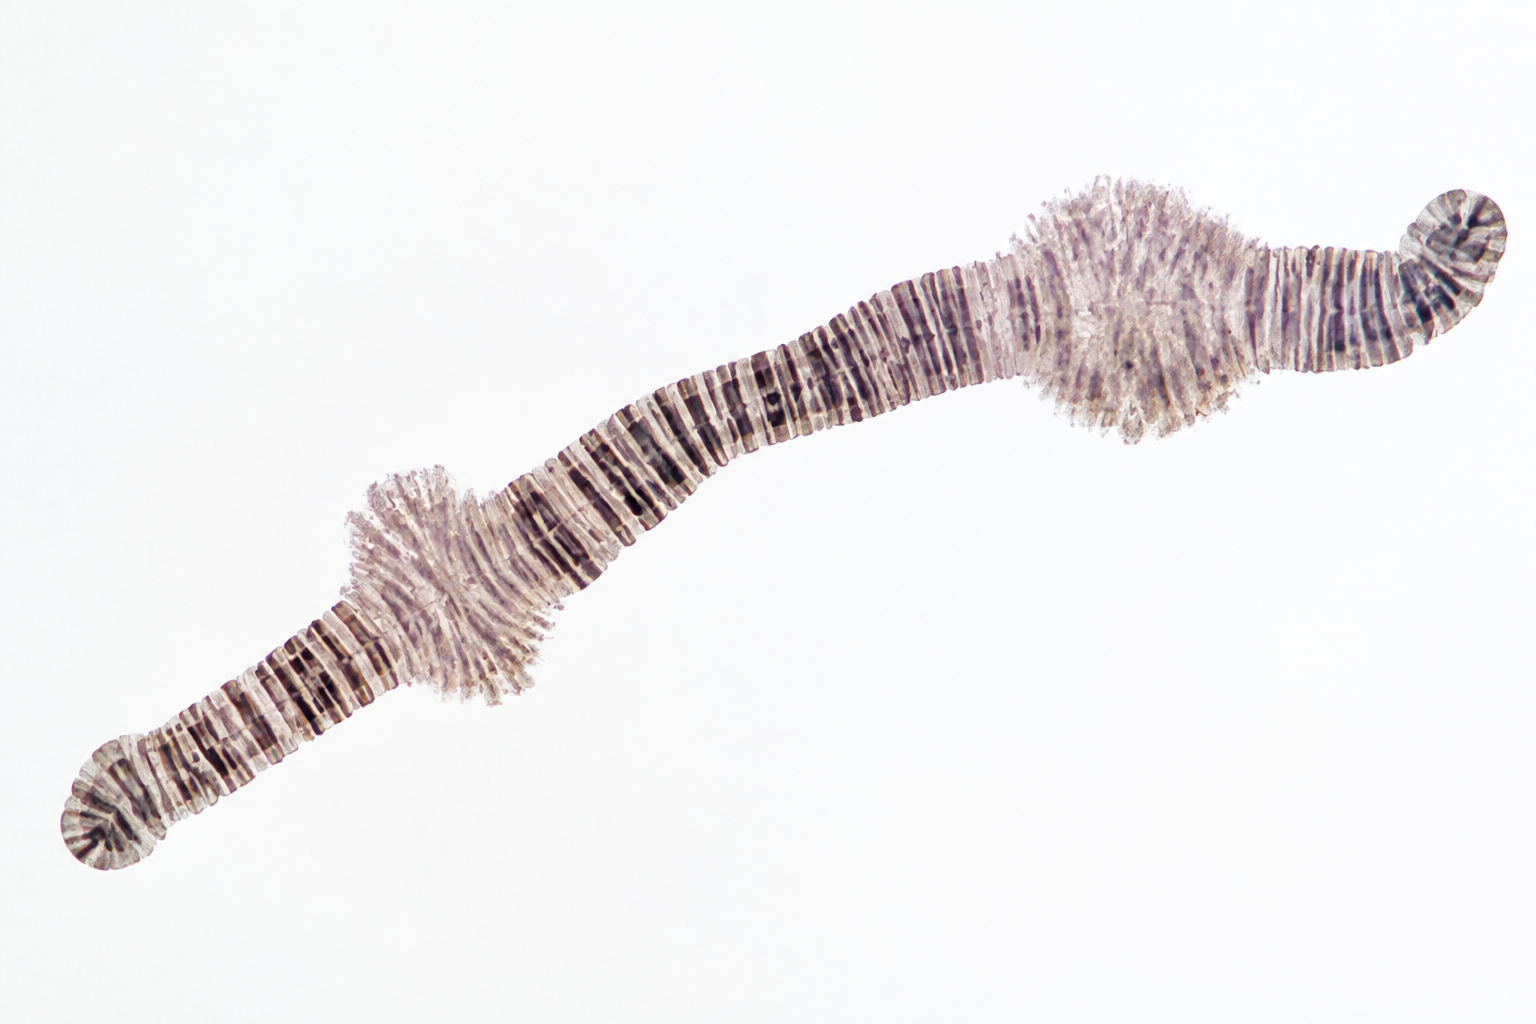
\includegraphics[width=0.56\linewidth]{images/book3/ai/b3-20-polytene-chromosome.png}

{\small A polytene \omterm{def:b1:genomes:genome}{chromosome} from a fly's salivary gland: banded,
with two puffs where the chromatin has opened for transcription.
Puffs appear and disappear as \omterm{def:b1:genomes:gene}{genes} are switched on and off.}
\end{omfigure}

\begin{example}[A signal becomes a pattern of expression]\label{ex:b1:expression-control:steroid}
Cortisol enters a liver \omterm{def:b1:cell-unit-of-life:cell}{cell} and binds its receptor, a \omterm{def:b1:expression-control:enhancer}{transcription
factor} kept inactive in the \omterm{def:b1:eukaryotic-cell:organelle}{cytosol}; the complex enters the nucleus,
binds a fifteen-base sequence present near a hundred \omterm{def:b1:genomes:gene}{genes} --- those of
\omterm{def:b1:biosyntheses-integration:gluconeogenesis}{gluconeogenesis} among them (\cref{ch:b1:biosyntheses-integration}) ---
and recruits acetylases and mediator: within an hour the \omterm{def:b1:enzymes:enzyme}{enzymes} of
glucose synthesis are being made. The same hormone in a lymphocyte,
whose open chromatin exposes a different set of those sequences,
switches on \omterm{def:b1:genomes:gene}{genes} that kill the \omterm{def:b1:cell-unit-of-life:cell}{cell}. One signal, one receptor, two
responses: the difference is which \omterm{def:b1:genomes:gene}{genes} were accessible.
\end{example}

\section{After transcription, and the making of a body}

\begin{proposition}[Control beyond the promoter]\label{prop:b1:expression-control:posttranscriptional}
\index{mRNA stability}
A \omterm{def:b1:cell-unit-of-life:prokeuk}{eukaryotic cell} also decides how a transcript is spliced
(alternative splicing gives a muscle and a brain different \omterm{def:b1:proteins:peptide}{proteins}
from one \omterm{def:b1:genomes:gene}{gene}), whether it is exported, how long it lasts (half-lives
from minutes for regulatory \omterm{def:b1:proteins:peptide}{proteins}' messages to days for
haemoglobin's, set by sequences in the untranslated regions that bind
\omterm{def:b1:proteins:peptide}{proteins} and small regulatory \omterm{def:b1:nucleic-acids:chain}{RNAs}), and whether it is translated
(iron-starved \omterm{def:b1:cell-unit-of-life:cell}{cells} block the translation of the ferritin message by a
\omterm{def:b1:proteins:peptide}{protein} bound to its $5'$ end, and release it when iron is present).
The \omterm{def:b1:proteins:peptide}{protein}, once made, is controlled by modification and degradation
(\cref{ch:b1:enzymes}). Each later level is faster and more local
than the one before, and more expensive: transcription decides what
the \omterm{def:b1:cell-unit-of-life:cell}{cell} can do, the later levels what it does now.
\end{proposition}

\begin{proposition}[Differential expression makes a body]\label{prop:b1:expression-control:differentiation}
\index{differentiation}
Every \omterm{def:b1:cell-unit-of-life:cell}{cell} of a multicellular \omterm{def:b1:organism-environment:organism}{organism} carries the same \omterm{def:b1:genomes:genome}{genome}; the
\omterm{def:b1:cell-unit-of-life:cell}{cells} differ because they express different subsets of it.
\emph{Housekeeping} \omterm{def:b1:genomes:gene}{genes} --- a few thousand for metabolism, the
\omterm{def:b1:gene-expression:ribosome}{ribosome}, the \omterm{def:b1:eukaryotic-cell:cytoskeleton}{cytoskeleton} --- are on in every \omterm{def:b1:cell-unit-of-life:cell}{cell}; the rest are
switched on in some \omterm{def:b1:cell-unit-of-life:cell}{cells} and off in others by the combinations of
\omterm{def:b1:expression-control:enhancer}{transcription factors} each \omterm{def:b1:cell-unit-of-life:cell}{cell} carries and the chromatin states it
has inherited. A red \omterm{def:b1:cell-unit-of-life:cell}{cell}'s precursor turns on globin and off nearly
everything else; a \omterm{def:b1:body-plans-tissues:nervous}{neuron} turns on its \omterm{def:b1:membranes-transport:transporters}{channels} and never divides
again. \emph{Differentiation} is the acquisition of a stable pattern
of expression, and \emph{development} (the Year 2 volume) is the
process by which signals between \omterm{def:b1:cell-unit-of-life:cell}{cells} set those patterns in the
right places.
\end{proposition}
\begin{proof}[Evidence]
A nucleus taken from a differentiated frog \omterm{def:b1:cell-unit-of-life:cell}{cell} and put into an egg
whose own nucleus has been removed can direct the development of a
whole tadpole (Gurdon, 1962; recalled from the High School volume): the
differentiated \omterm{def:b1:cell-unit-of-life:cell}{cell} had lost no \omterm{def:b1:genomes:gene}{genes}, only switched them off, and the
egg's \omterm{def:b1:cell-unit-of-life:cell}{cytoplasm} reset the switches. The \omterm{def:b1:proteins:peptide}{proteins} of a \omterm{def:b1:cell-unit-of-life:cell}{cell} type,
separated on a gel, differ from another type's; its messengers, once
sequenced, are a subset of the \omterm{def:b1:genomes:genome}{genome} specific to it; and a handful of
\omterm{def:b1:expression-control:enhancer}{transcription factors} introduced into a skin \omterm{def:b1:cell-unit-of-life:cell}{cell} can reprogram it
into a stem \omterm{def:b1:cell-unit-of-life:cell}{cell} or a \omterm{def:b1:body-plans-tissues:nervous}{neuron}.
\end{proof}

\begin{example}[A gene read in two organs]\label{ex:b1:expression-control:twoorgans}
The \omterm{def:b1:genomes:gene}{gene} for the \omterm{def:b1:enzymes:enzyme}{enzyme} that makes glucose from glucose-6-phosphate
is expressed in the liver and the kidney and in no other \omterm{def:b1:body-plans-tissues:tissue}{tissue}: its
promoter carries sites for factors present only there, and in other
\omterm{def:b1:cell-unit-of-life:cell}{cells} its promoter is methylated and its chromatin closed. A muscle,
which carries the \omterm{def:b1:genomes:gene}{gene} intact, cannot release glucose into the blood
(\cref{ch:b1:biosyntheses-integration}) --- not for lack of the \omterm{def:b1:genomes:gene}{gene}
but because the \omterm{def:b1:genomes:gene}{gene} is not read. The \omterm{def:b1:genomes:genome}{genome} is the same; the
expression is the \omterm{def:b1:mammal-organization:organ}{organ}.
\end{example}

\section{Exercises}

\begin{exercise}[$\star$]\label{exo:b1:expression-control:1}
Name the elements of the \omterm{def:b1:expression-control:operon}{lac operon} and give the state of the \omterm{def:b1:expression-control:operon}{operon}
with and without lactose, with and without glucose.
\end{exercise}

\begin{exercise}[$\star$]\label{exo:b1:expression-control:2}
Explain the difference between a \omterm{def:b1:genomes:gene}{gene} product that acts in trans and
a site that acts in cis, with one example of each from the \omterm{def:b1:expression-control:operon}{operon}.
\end{exercise}

\begin{exercise}[$\star$]\label{exo:b1:expression-control:3}
From the \omterm{def:b1:expression-control:cap}{diauxie} figure, read the duration of the lag and the
doubling times on each sugar.
\end{exercise}

\begin{exercise}[$\star$]\label{exo:b1:expression-control:4}
Define \omterm{def:b1:expression-control:enhancer}{enhancer}, \omterm{def:b1:expression-control:enhancer}{transcription factor} and housekeeping \omterm{def:b1:genomes:gene}{gene}.
\end{exercise}

\begin{exercise}[$\star\star$]\label{exo:b1:expression-control:5}
Give the phenotype (inducible, constitutive, uninducible) of: $I^-$;
$O^c$; $I^s$; $I^-\,O^+\,Z^+ / I^+\,O^+\,Z^+$; $I^s\,O^+\,Z^+ /
I^+\,O^+\,Z^+$; $I^+\,O^c\,Z^- / I^+\,O^+\,Z^+$.
\end{exercise}

\begin{exercise}[$\star\star$]\label{exo:b1:expression-control:6}
Compare the lac and \omterm{prop:b1:expression-control:trp}{trp operons}: what the small molecule does to the
\omterm{def:b1:expression-control:operon}{repressor} in each, and why the logic is opposite.
\end{exercise}

\begin{exercise}[$\star\star$]\label{exo:b1:expression-control:7}
A mutant cannot make cAMP. Predict its growth on glucose, on lactose
alone, and on both, and the level of $\beta$-galactosidase in each
case.
\end{exercise}

\begin{exercise}[$\star\star$]\label{exo:b1:expression-control:8}
Explain why attenuation is impossible in eukaryotes, from the
architecture of the \omterm{def:b1:cell-unit-of-life:prokeuk}{eukaryotic cell}.
\end{exercise}

\begin{exercise}[$\star\star$]\label{exo:b1:expression-control:9}
An \omterm{def:b1:expression-control:enhancer}{enhancer} is moved from \qty{5}{kb} upstream of its \omterm{def:b1:genomes:gene}{gene} to
\qty{5}{kb} downstream and inverted; the \omterm{def:b1:genomes:gene}{gene} is still expressed.
Explain what this shows about how \omterm{def:b1:expression-control:enhancer}{enhancers} work.
\end{exercise}

\begin{exercise}[$\star\star\star$]\label{exo:b1:expression-control:10}
Five thousand $\beta$-galactosidase tetramers of \qty{4096}{}
residues cost how many \omterm{def:b1:water-small-molecules:atp}{ATP} (four per residue)? A \omterm{def:b1:cell-unit-of-life:cell}{cell}'s budget per
generation is about \qty{1e10}{} \omterm{def:b1:water-small-molecules:atp}{ATP}. Compute the growth
disadvantage of a constitutive mutant, and the number of generations
for its share of a mixed population to fall from a half to a
hundredth.
\end{exercise}

\begin{exercise}[$\star\star\star$]\label{exo:b1:expression-control:11}
A liver \omterm{def:b1:cell-unit-of-life:cell}{cell} and a \omterm{def:b1:body-plans-tissues:nervous}{neuron} of the same person are compared: same
\omterm{def:b1:genomes:genome}{genome}, different \omterm{def:b1:proteins:peptide}{proteins}, and each division of the liver \omterm{def:b1:cell-unit-of-life:cell}{cell}
gives liver \omterm{def:b1:cell-unit-of-life:cell}{cells}. Explain, with chromatin, factors and inheritance of
marks, how the difference is made and how it is maintained.
\end{exercise}

\begin{exercise}[$\star\star\star$]\label{exo:b1:expression-control:12}
"A bacterium reads its environment; a \omterm{def:b1:cell-unit-of-life:cell}{cell} of a body reads its
history." Discuss in a paragraph the two kinds of control, their
signals, their timescales and their reversibility.
\end{exercise}

\section{Problem: Diauxie}

\begin{problem}[{Weekend problem --- Monod's two-phase growth curve
reconstructed cell by cell: glucose exhausted, lactose induced,
enzymes counted, mutants predicted and the cost of regulation
reckoned, ending on the induction factor of $\beta$-galactosidase}]
\label{pb:b1:expression-control:1}
A culture of \emph{E. coli} starts at $10^7$ \omterm{def:b1:cell-unit-of-life:cell}{cells} per millilitre in
a medium with \qty{0.5}{mmol/L} of glucose and \qty{1.0}{mmol/L} of
lactose. On glucose the \omterm{def:b1:cell-unit-of-life:cell}{cells} double every \qty{20}{min}, on lactose
every \qty{30}{min}; a \omterm{def:b1:cell-unit-of-life:cell}{cell} needs \qty{1.5e-12}{g} of sugar per
division (\qty{180}{g/mol} of glucose; lactose, \qty{342}{g/mol},
counts as two glucoses). Uninduced \omterm{def:b1:cell-unit-of-life:cell}{cells} hold 5 molecules of
$\beta$-galactosidase; fully induced, \num{5000}. Induction takes
\qty{30}{min}. The \omterm{def:b1:enzymes:enzyme}{enzyme} is a tetramer of $4\times 1024$ residues;
each residue costs 4 \omterm{def:b1:water-small-molecules:atp}{ATP}; a \omterm{def:b1:cell-unit-of-life:cell}{cell}'s \omterm{def:b1:water-small-molecules:atp}{ATP} budget is $10^{10}$ per
division and its \omterm{def:b1:proteins:peptide}{protein} $\num{1.5e-13}{g}$ (\qty{110}{Da} per residue).

\medskip
\noindent\textbf{Part I --- The glucose phase.}
\begin{enumerate}
  \item Compute the glucose available per millilitre, in grams.
  \item How many divisions per millilitre can it support?
  \item Starting from $10^7$ \omterm{def:b1:cell-unit-of-life:cell}{cells}, how many \omterm{def:b1:cell-unit-of-life:cell}{cells} are there when the
        glucose runs out? (A division makes one new \omterm{def:b1:cell-unit-of-life:cell}{cell}.)
  \item How many doublings is that, and how long does the glucose
        phase last?
  \item During this phase, what is the state of the \omterm{def:b1:expression-control:operon}{lac operon}, and
        why, in molecular terms (\omterm{def:b1:expression-control:operon}{repressor} and CAP)?
\end{enumerate}

\medskip
\noindent\textbf{Part II --- The switch.}
\begin{enumerate}[resume]
  \item When the glucose is gone, what rises inside the \omterm{def:b1:cell-unit-of-life:cell}{cells} and
        what does it bind?
  \item Lactose was present all along. Why was the \omterm{def:b1:expression-control:operon}{operon} nevertheless
        almost off during the glucose phase?
  \item During the \qty{30}{min} lag each \omterm{def:b1:cell-unit-of-life:cell}{cell} makes its \num{5000}
        \omterm{def:b1:enzymes:enzyme}{enzymes}. Compute the \omterm{def:b1:enzymes:enzyme}{enzyme} molecules made per second per
        \omterm{def:b1:cell-unit-of-life:cell}{cell}, and the residues per second.
  \item A \omterm{def:b1:cell-unit-of-life:cell}{cell} holds \num{20000} \omterm{def:b1:gene-expression:ribosome}{ribosomes} at \qty{20}{} residues per
        second. What fraction of its translation is devoted to
        $\beta$-galactosidase during the lag?
  \item Compute the mass of \num{5000} tetramers and the fraction of
        the \omterm{def:b1:cell-unit-of-life:cell}{cell}'s \omterm{def:b1:proteins:peptide}{protein} they represent.
  \item Compute the induction factor.
  \item Why is the permease (\emph{lacY}) as necessary as the \omterm{def:b1:enzymes:enzyme}{enzyme}
        for growth on lactose, and what happens to a \emph{lacY}$^-$
        mutant given lactose?
\end{enumerate}

\medskip
\noindent\textbf{Part III --- The lactose phase.}
\begin{enumerate}[resume]
  \item Compute the lactose available per millilitre in glucose
        equivalents, in grams.
  \item How many further divisions does it support, and what is the
        final \omterm{def:b1:cell-unit-of-life:cell}{cell} count?
  \item How long does the lactose phase last?
  \item Draw up the timeline: glucose phase, lag, lactose phase, total.
  \item Explain why the doubling time is longer on lactose (two
        reasons: one about the \omterm{def:b1:enzymes:enzyme}{enzyme} step, one about the permease).
\end{enumerate}

\medskip
\noindent\textbf{Part IV --- Mutants and costs.}
\begin{enumerate}[resume]
  \item An $I^-$ mutant: describe its growth curve on the same medium
        and its \omterm{def:b1:enzymes:enzyme}{enzyme} level throughout.
  \item A CAP$^-$ mutant: describe its curve and \omterm{def:b1:enzymes:enzyme}{enzyme} level.
  \item An $O^c$ mutant in a medium with lactose only: any difference
        from wild type? And with glucose only?
  \item Compute the \omterm{def:b1:water-small-molecules:atp}{ATP} cost per generation of making \num{5000}
        tetramers, and the fraction of the \omterm{def:b1:cell-unit-of-life:cell}{cell}'s budget.
  \item If that fraction lengthens the generation time by the same
        fraction, by how much does the $I^-$ mutant's growth rate lag
        the wild type's on glucose?
  \item Starting at equal numbers, after how many generations on
        glucose is the mutant one tenth of the population? ($r^n =
        0.1/0.9$ with $r$ the ratio of growth rates per generation,
        i.e.\ $2^{-\delta}$ for a lag $\delta$ in doublings.)
  \item Explain why, nevertheless, $I^-$ mutants are common in
        laboratory strains grown on lactose.
  \item State the result: the induction factor of
        $\beta$-galactosidase, the cost of making it unnecessarily as
        a fraction of the \omterm{def:b1:water-small-molecules:atp}{ATP} budget, and the total time of the
        diauxic experiment.
\end{enumerate}
\end{problem}
